

\subsection{Xử lý hình ảnh Python}
Module xử lý hình ảnh bằng Python nhận luồng video từ camera ESP32-CAM hoặc webcam, sau đó sử dụng TensorFlow Lite để phát hiện người và trích xuất các điểm khớp (skeleton) theo thời gian thực.  

Quy trình xử lý bao gồm:
\begin{itemize}
    \item Khởi tạo pipeline nhận luồng video từ camera.  
    \item Tiền xử lý khung hình (chuẩn hóa kích thước, màu sắc).  
    \item Chạy mô hình học máy TensorFlow Lite để phát hiện và trích xuất các điểm khớp của cơ thể người.  
    \item Vẽ skeleton trực quan trên khung hình để theo dõi trạng thái và chuyển động.  
\end{itemize}

Kết quả thực nghiệm cho thấy module hoạt động ổn định, xử lý khung hình theo thời gian thực với tốc độ trung bình 3--5 FPS.  
Hình~\ref{fig:python_skeleton} minh họa giao diện theo dõi người và skeleton được module xử lý hình ảnh tạo ra trong quá trình chạy thử nghiệm.

\begin{figure}[H]
    \centering
    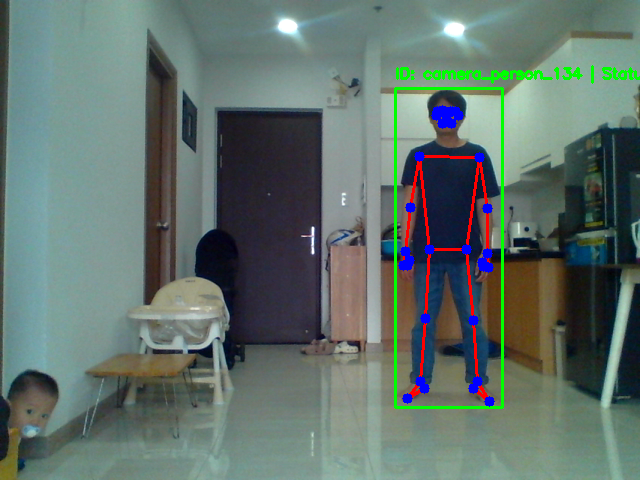
\includegraphics[width=0.85\textwidth]{figures/fall_detection_screen_shoot.png}
    \caption{Module Python xử lý hình ảnh: phát hiện người và vẽ skeleton theo thời gian thực.}
    \label{fig:python_skeleton}
\end{figure}
\subsection{Module nhận diện hình ảnh (Python)}
\label{sec:python_vision}

Module máy chủ xử lý được xây dựng bằng Python nhằm thực hiện các chức năng: thu nhận luồng dữ liệu từ camera, triển khai mô hình học sâu để dựng khung xương (skeleton), đồng thời tích hợp với hệ thống gửi cảnh báo qua MQTT và Telegram. Ngoài ra, module còn ghi log vào cơ sở dữ liệu SQLite và duy trì kết nối với Asterisk Management Interface (AMI).  

\begin{figure}[H]
    \centering
    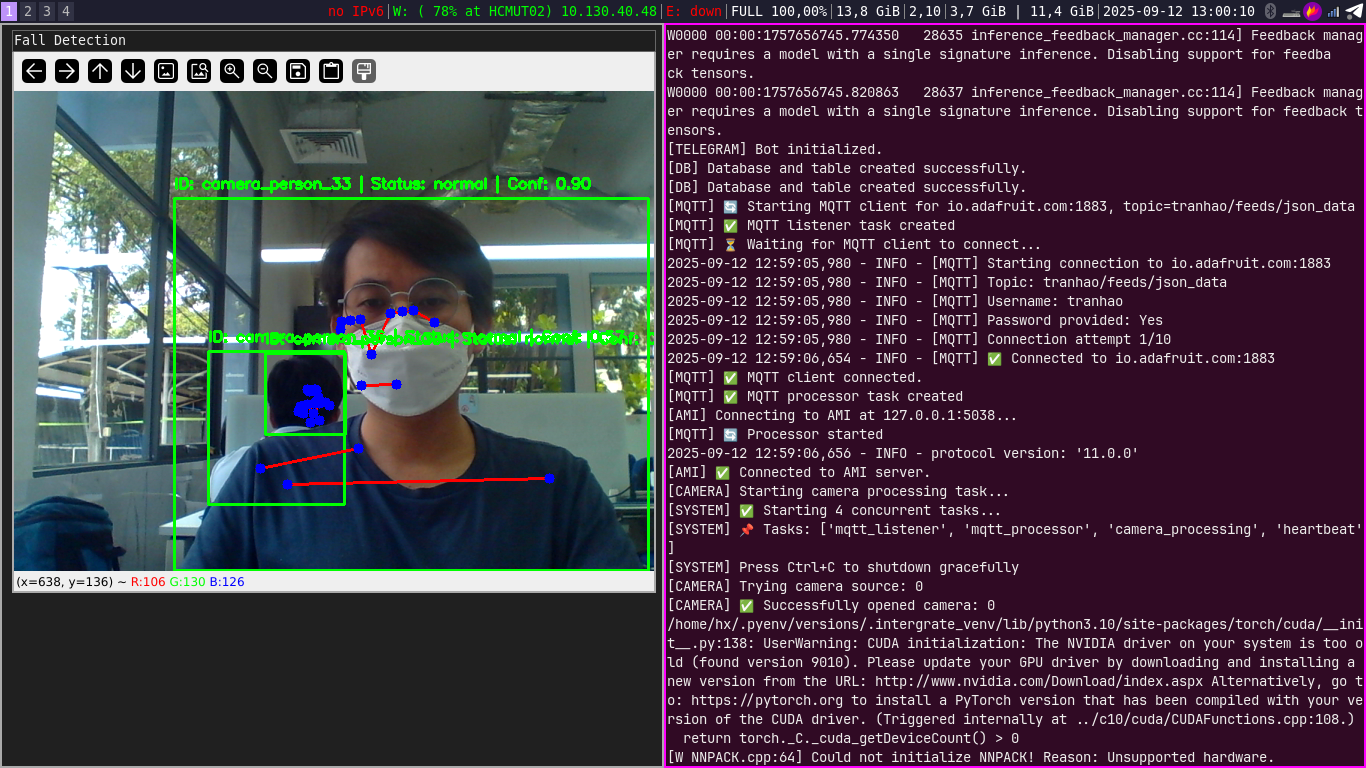
\includegraphics[width=0.8\textwidth]{figures/python_runing_log.png}
    \caption{Log thực nghiệm: Python xử lý ảnh và điều phối các tác vụ.}
    \label{fig:python_runing_log}
\end{figure}

\textbf{Kết luận:} Module Python đã hoạt động đúng chức năng, bảo đảm khả năng thu nhận dữ liệu camera, chạy nhận diện hình ảnh, đồng bộ dữ liệu qua MQTT, và kích hoạt các kênh cảnh báo. Hệ thống tuy có hạn chế về hỗ trợ CUDA (do phiên bản driver cũ) nhưng không ảnh hưởng đến quá trình thực thi trên CPU.

\subsection{Thử nghiệm Asterisk Call/SMS Gateway}
\label{sec:asterisk_test}

Trong hệ thống, Asterisk được sử dụng như một cổng trung gian để gửi cảnh báo bằng SMS và có tiềm năng mở rộng sang chức năng gọi điện tự động.  
Trong quá trình thử nghiệm, việc kích hoạt nhắn tin SMS qua Asterisk hoạt động thành công, cho phép hệ thống gửi cảnh báo đến số điện thoại đã đăng ký.  

Tuy nhiên, chức năng gọi thoại chưa được triển khai ổn định. Khi thay đổi máy chủ Asterisk, cấu hình giữ nguyên nhưng khả năng khởi tạo và duy trì cuộc gọi không đồng nhất. Điều này cho thấy còn tồn tại sự phụ thuộc vào môi trường triển khai, cần được nghiên cứu và tối ưu thêm trong tương lai.  

\begin{figure}[H]
    \centering
    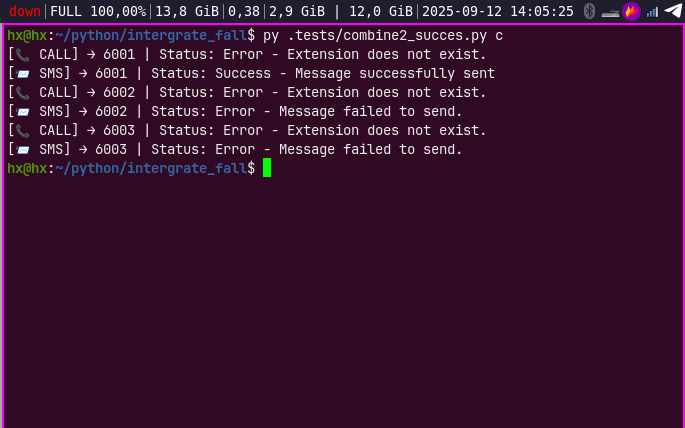
\includegraphics[width=0.8\textwidth]{figures/ast_call_sms_test.png}
    \caption{Thử nghiệm gửi SMS cảnh báo qua Asterisk.}
    \label{fig:ast_call_sms_test}
\end{figure}

\textit{Kết luận:} Module Asterisk đã hỗ trợ thành công chức năng nhắn tin SMS trong hệ thống. Chức năng gọi thoại vẫn còn hạn chế và sẽ cần nghiên cứu bổ sung để đảm bảo tính ổn định khi triển khai thực tế.

\subsection{Kênh cảnh báo Telegram}
\label{sec:telegram_alert}

Hệ thống Telegram Bot đóng vai trò là kênh cảnh báo trực quan, giúp gửi thông báo đến người dùng ngay khi phát hiện té ngã.  
Cơ chế hoạt động được chia thành hai hướng:
\begin{itemize}
    \item \textbf{Từ module phần cứng (ESP32 + 4G/GPS):} Khi xảy ra sự kiện té ngã, bản tin MQTT hoặc SMS được phát ra từ thiết bị. Hệ thống trung tâm sau đó chuyển tiếp nội dung này đến người dùng thông qua Telegram.
    \item \textbf{Từ module xử lý hình ảnh (Python):} Khi nhận diện được té ngã qua camera và skeleton, hệ thống Python trực tiếp gửi cảnh báo đến Telegram, kèm thông tin chi tiết.
\end{itemize}

\begin{figure}[H]
    \centering
    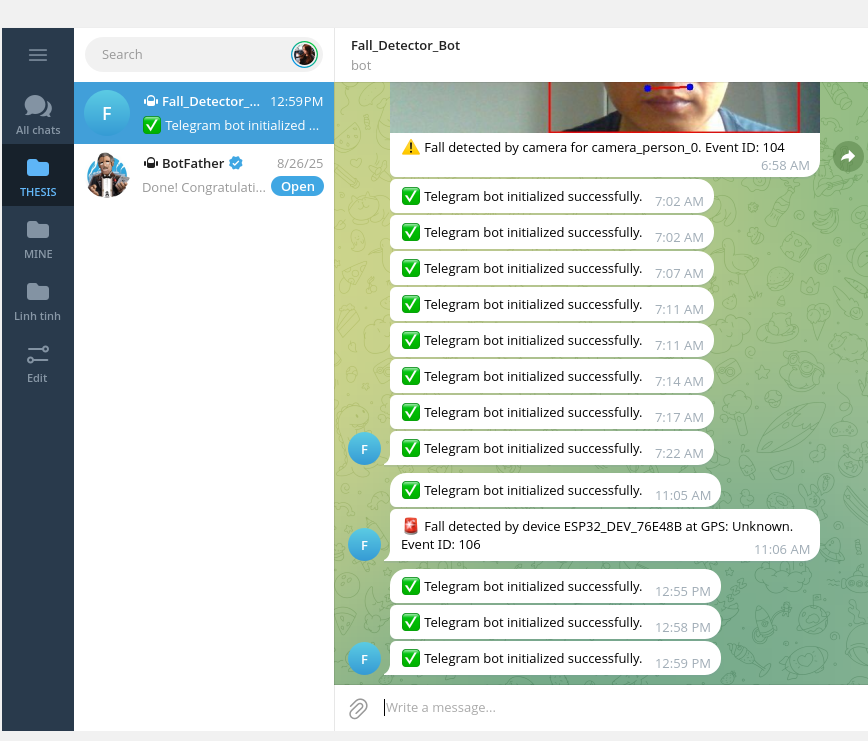
\includegraphics[width=0.8\textwidth]{figures/telegram_fall_module1_send.png}
    \caption{Thông báo cảnh báo té ngã từ module phần cứng (ESP32) qua Telegram.}
    \label{fig:telegram_hw}
\end{figure}

\begin{figure}[H]
    \centering
    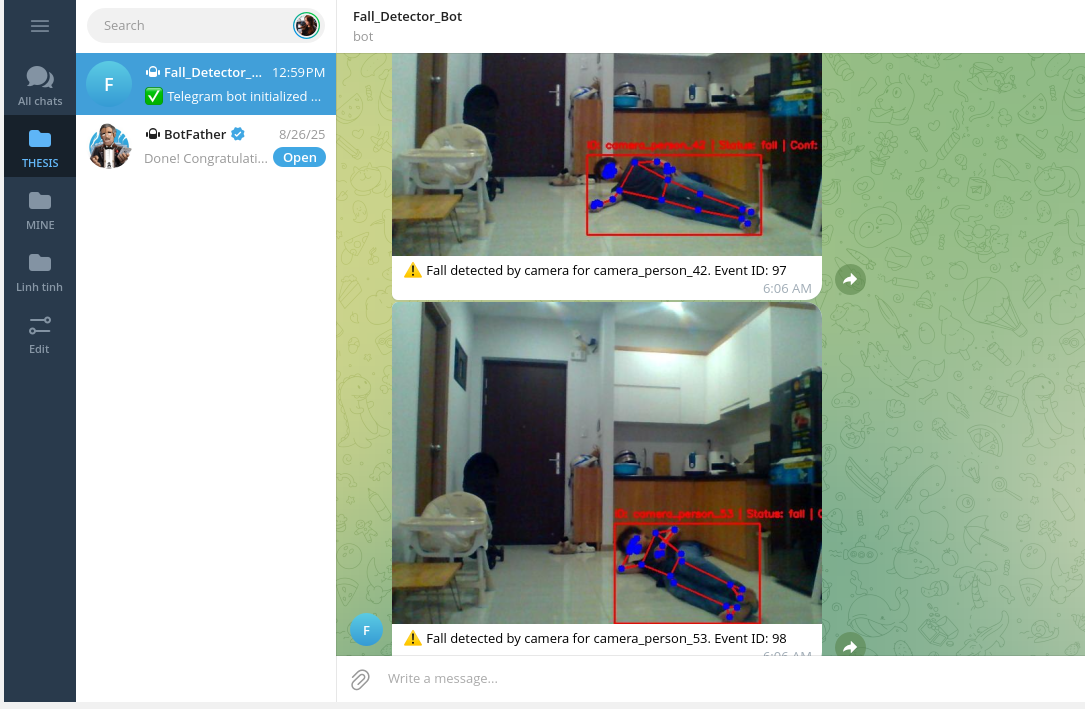
\includegraphics[width=0.8\textwidth]{figures/telegram_python_fall_send.png}
    \caption{Thông báo cảnh báo té ngã từ module xử lý hình ảnh Python qua Telegram.}
    \label{fig:telegram_python}
\end{figure}

\textit{Kết luận:} Kênh Telegram đã hoạt động ổn định, đóng vai trò cầu nối giữa hệ thống phát hiện té ngã và người dùng cuối. Việc kết hợp cả hai nguồn cảnh báo (thiết bị phần cứng và module xử lý hình ảnh) giúp tăng độ tin cậy và giảm thiểu khả năng bỏ sót sự kiện.
